\chapter{RISC-V and CV32E40P Core}{
	% Article & books
	% INTRO
	RISC-V is a free and open Instruction Set Architecture (ISA) with a small instruction set (Reduced Instruction Set Computer) at the heart of core of a System On Chip (SOC).
	An ISA is the abstract description of core instruction, registers, data types and extension, without design imposition. 
	Many implementation of a CPU can rely on the same ISA  using different design, in this way software used in these different implementation could be equal.
	RISC-V can be seen a first try to standardize the Instruction Set world without using new technology.
	The focus is on modular approach and extensibility in order to increase field of use of the ISA.
    
    For these reasons the use of a free and open ISA worldwide unlock partially software from hardware implementation since the interface is always about equal.
    This subdivision speed up computer CPU progress with lower efforts in software support.
    Indeed companies efforts can be focused more on design and less on software support since the interface is the same.\\
    
    RISC-V is maintained by the RISC-V foundation born in 2015, it is driven by open collaboration in order to improve RISC-V ISA.
    The use of free and open collaboration speed up bug resolution, reduce design risk and lead to speed up in design techniques.
    In order to be used worldwide the RISC-V architecture use a Reduced Instruction Set  of 47 Base Instruction, the ISA is designed with a modular approach to easily add extensions. 
    In this way the ISA can be used for whatever application since the core can be customized according to application and field of use.
    It is already used in computer, supercomputer, embedded application and it now supports by many Operative System like RTOS and Linux.\\
    
    It is precisely the fact that it can be customized that increase the worldwide use.
    This increase the test done on the ISA implementation which lead to ISA improvement and increase the ISA dependability.
    
    Starting from these ideas we could summarized some benefits of a open and free ISA \bscite{Asanovic2014} :
    \begin{itemize}
        \item \textbf{Greater Innovation:} More people working on the same ISA speed up innovation;
        \item \textbf{Shared Open Core Design:} with a free ISA the implementation (e.g. System Verilog design) can be shared as open source, this prevent malicious traps doors and increase transparency, it also allows the born of new industries that create products from open design;
        \item \textbf{Cheaper Processors:} the reduction of company work on software stack decrease the processors cost, this speed up widespread of IoT;
        \item \textbf{Longevity of Software Stack:} a standard ISA allow the creation of an endurance Software Stack since it don't depends to a company;
        \item \textbf{Architecture Education and Research closer to real application: } the academic world could work on open hardware and software.
    \end{itemize}
    
    At 2020 the 23\% of ASICs and FPGAs project incorporate at least one RISC-V core and it is foreseen that in 2025 will be used 62.4 Billion of RISC-V Cores respect to 10 Billion of 2020.
    This is surely a positive sign of open ISA strategy, it means that many industries are rely on RISC-V ISA architecture and they use it to speed up their internal design.
    
	
	\section{History}{
	    ISA of RISC-V started in 2010 in a project for the Parallel Computing Laboratory (Par Lab) at Berkeley held by Prof. Krste Asanović and graduate students Yunsup Lee and Andrew Waterman.
	    The idea of RISC-V ISA born to create a complete open hardware ecosystem, indeed until that moment the main ISA was proprietary and academic world work on non realistic architecture.
	    Anyway the outcome of an open ISA also help industries since the main costs an complexity in the creation of a new chip is the development of software stack for new ISAs.
	    Indeed any change to the ISA means redevelop some parts of software with high costs.
	    Due to historical reason ISAs are proprietary, but in the last 40 years no meaningful development arise in this field and so there aren't no meaning to avoid ISA standardization. 
	    Starting from this ideas the RISC-V project begin and was developed up to now.\\
	    
	    The first release of RISC-V ISA was in 2011 and it was under the Berkeley Software Distribution (BSD) license. 
	    After some year of RISC-V use and some publication \bscite{Asanovic2014} in 2011 was created the first chip in 28nm FDSOI and in 2015 was held the first RISC-V workshop, in the same year was founded the RISC-V foundation with 36 members \bscite{RISCVHistory}.
	    
	    In the following year the RISC-V ISA was put under Creative Common license in order to enable an easy use and open contribution.\\
	    
	    In the year 2013-3018 in the UC Berkeley ASPIRE Lab was created many RISC-V compatible free processors, today RISC-V Foundation continue to support RISCV ISA standardization helping industries to use it, the versions of the ISA is now frozen at 2019  in order to simplify development of RISCV core. 
	    These are the official ISA  standard: \href{https://github.com/riscv/riscv-isa-manual/releases/download/Ratified-IMFDQC-and-Priv-v1.11/riscv-privileged-20190608.pdf}{RISCV-privileged} and  \href{https://github.com/riscv/riscv-isa-manual/releases/download/Ratified-IMAFDQC/riscv-spec-20191213.pdf}{RISCV-unprivilged}. 
	    Instead in this page you can find all original standard documents: \href{https://riscv.org/technical/specifications/}{RISCV-spec}.
	}% end History 

	\section{RISC-V ISA}{
	    RISC-V ISA is described in two document:
	    \begin{itemize}
	        \item \textbf{riscv-privileged:} Or Kernel mode, in this document are described privileged  instructions any attempt to execute this instruction from User Mode will not be executed and it is considered illegal instructions. These are the instructions used in the Operative System to perform operations.
	        \item \textbf{riscv-unprivileged:} Or Non privileged mode, it is made by all instructions that can be run only in user mode.
	    \end{itemize}
	    
	    In these two documents the ISA is described avoiding implementations details as much as possible. At the beginning of the standards are defined some terms \bscite{RISCV_unprivileged}:
	    
	    \begin{itemize}
	        \item \textbf{core:} An architecture is defined a core if it contains an instruction fetch; 
	        \item \textbf{harts:} Are hardware threads that can be support by the ISA, a RISC-V compatible core can supports multiple harts;
	        \item \textbf{coprocessor:} It is an instruction set extension used by the RISC-V compatible core, this coprocessor is considered as a separate unit that is controlled by a RISC-V instruction flux but it have relative autonomy respect to primary RISC-V core, this is an example of RISC-V coprocessor programming for sensor reading \href{https://github.com/espressif/esp-idf/blob/c13afea635adec735435961270d0894ff46eef85/docs/en/api-guides/ulp-risc-v.rst}{RISC-V sensors};
	        \item \textbf{accelerator:} This component are really useful to perform specialized complex task, e.g. I/O and AI accelerator, the first manage I/O processing task while the second could be a voice recognition AI.
	    \end{itemize}
	    As you can see RISC-V can have extensions and coprocessors, it can also have many system-level organizations; single-core, many-core shared memory and so on.
	    
	    
	    A RISC-V ISA implementation must contain base integer ISA, starting from this basis can be added optional extensions. 
	    The base integer ISA is enough to support a compilers, assemblers, linkers, and operating system, in this way it provide a starting point to custom implementations.\\
	    
	    The RISC-V ISA is divided in four base ISA family and it is "designed to support extensive customization and specialization" \bscite{RISCV_unprivileged}, each family is distinguished by a different register width and the number of corresponding address space. 
	    The four family are RV32I, RV32E (with 32 bits) RV64I (64 bits) and RV128I (128 bits), naturally 128 bits is a huge number of address, anyway RISC-V standard want to be prepared for future huge computer address. These four ISA are considered four base ISA, in this way e.g RV64I shouldn't be compliant with RV32I and so have separate implementation.\\
	     
	    
	    In addition to base ISA (marked with I suffix for Integer) there are some standard extension:
	    \begin{itemize}
	        \item \textbf{M:} It is the standard integer multiplication and division extension;
	        \item \textbf{A:} It is the standard Atomic instruction extension that add some instruction able to "atomically read, modify, and write memory  for  inter-processor  synchronization" \bscite{RISCV_unprivileged};
	        \item \textbf{F:} It is the standard floating point extension;
	        \item \textbf{D:} It is the standard double precision floating point extension;
	        \item \textbf{C:} It is the standard compressed instruction extension that provide the 16 bit form of common instructions.
	   \end{itemize}
	   

	   The memory of a RISC is a single byte-addressable address space of $2^{XLEN}$ bytes, a word is 32 bits, an halfword 16 bits, a doubleword 64 bits and a quadword 128 bits. 
	   The memory accesses can be done using \textit{explicit} and \textit{implicit} mode, the first is used by load and store instruction while the second is used in instruction fetch to give the encoded instruction to execute.
	   Only some section of the memory can be used, these sections create the \textit{execution environment}, if an instruction try to read/write outside of this zone, an exception is raised.\\
	   
	   Each base instruction for the RISC-V ISA have 32-bit aligned to the 32-bit boundaries, anyway are also supported variable length instruction like 16-bit compressed instruction aligned to the 16-bit boundary, for these instruction is needed the compressed decoder block in the Instruction Fetch stage.
	   The term IALIGN refers to the instruction address alignment of the ISA, it could be only 32 or 16 bit. Instead the term ILEN refers to the maximum instuction lenght bit.\\
	    \begin{figure}[H]
			\centering
			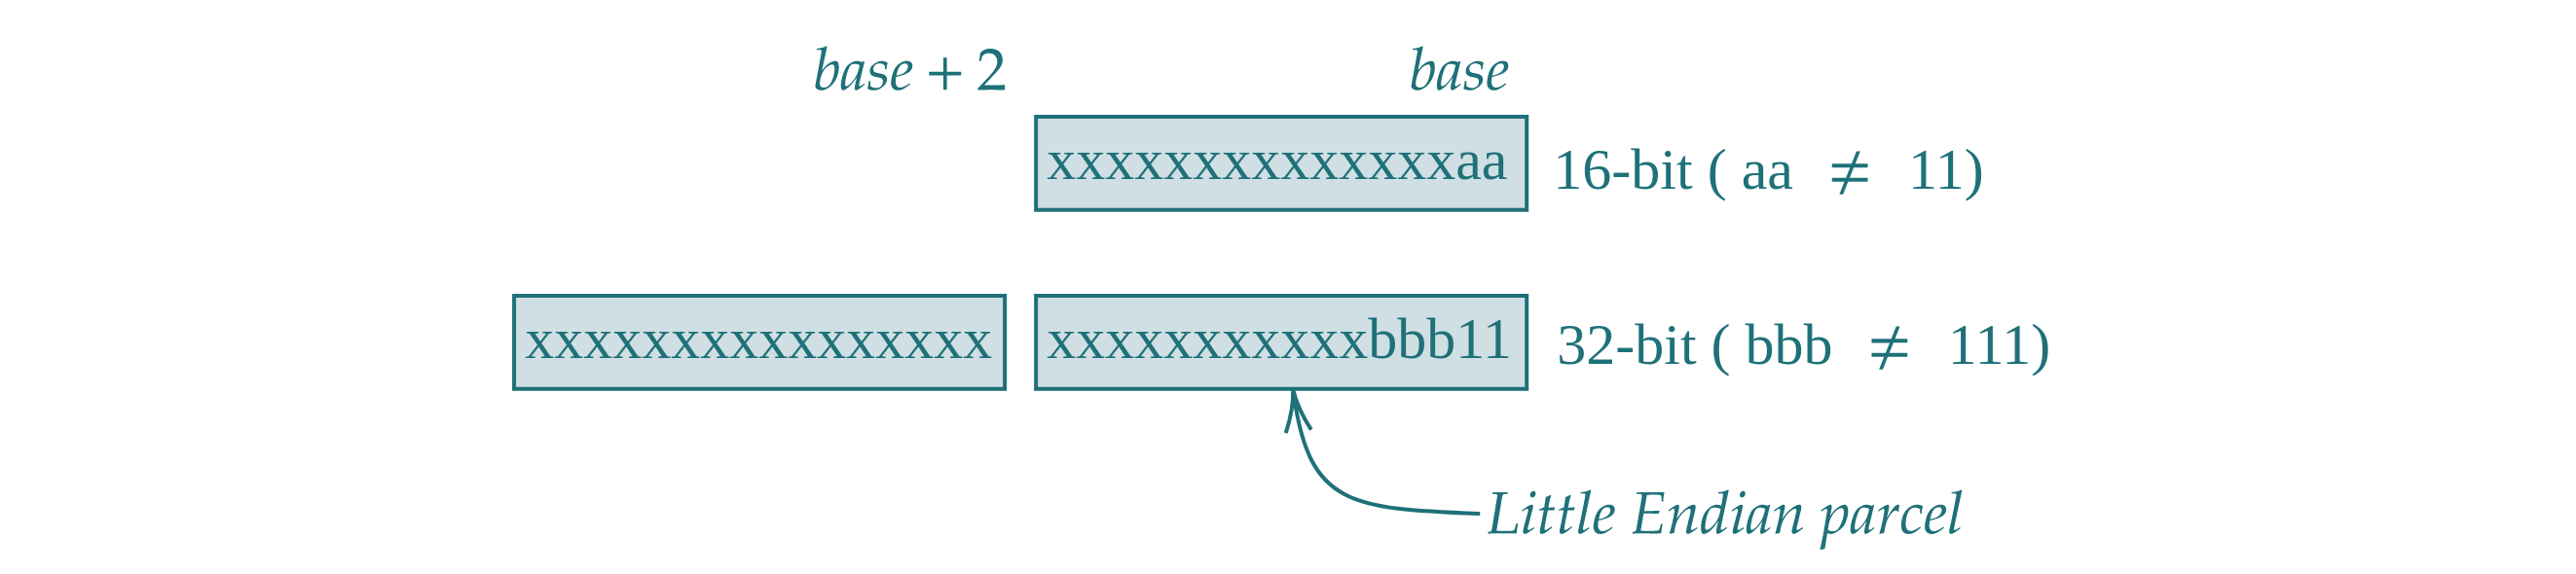
\includegraphics[scale=0.18,center]{./images/RISCVinstruction.png}
			\caption{32-bit and 16 bit instruction, frozen in the last release.}
			\label{fig:riscvinstruction}
		\end{figure}  
		The lowest two bit [1:0] on the right are used to recognize a compressed instruction, if they are both 1 the instruction isn't compressed, othewise it is compressed.
		
		Even if the RISC-V can have either Little-Endian and Big-Endian memory order, the instruction is divided in 16-bit Little-Endian parcels, the parcels of the same instruction is saved contiguously with the lowest-addressed parcel in the lowest-numbered bits in the instruction.
		
		\subsection{Base Instructions}{
		    We will discuss the RV32I base version since in this Master Thesis we use the CV32E40P core.
		    For RV32I  ISA we have 32 unprivileged registers where the first is hardwired to 0 and the others are general purpose, there is also the 32 bit Program Counter register.
		    
		    The base instructions used are six R/I/S/B/U/J and are shown in figure \ref{fig:riscv_instruction_format}, all 47 base instruction is encoded using these 6 format.
		    As you can see many parameters have the same place, this enable an easier decode of instructions and so increase low power behaviour of possible implementations.
    	    \begin{figure}[H]
    			\centering
    			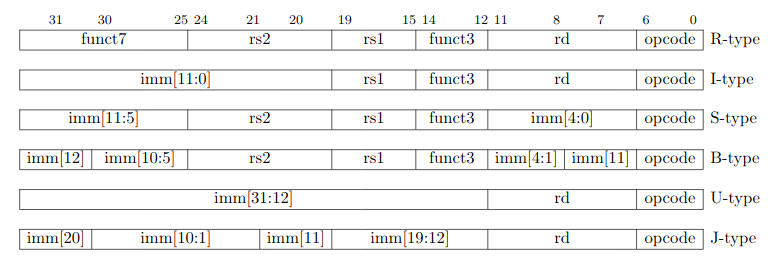
\includegraphics[scale=0.55,center]{./images/riscv_instruction_format.png}
    			\caption{RISC-V ISA instruction format.}
    			\label{fig:riscv_instruction_format}
    		\end{figure}
    		
    		Inside the table \ref{fig:riscv_instruction_format} in the field you can see: \textit{opcode} that is the operation code, \textit{rd} that is the number of register destination, \textit{immediate} that is a constant value or the offset for an address, \textit{func3} that is an additional opcode of 3 bit, \textit{func7} that is an additional opcode of 7 bit, \textit{rs1 \& rs2} that are the first and the second source register number.\\
		}%end Base Instructions
		
		In figure \ref{fig:riscv_architecture1} there is an implementation of the RISCV ISA.
	    \begin{figure}[H]
			\centering
			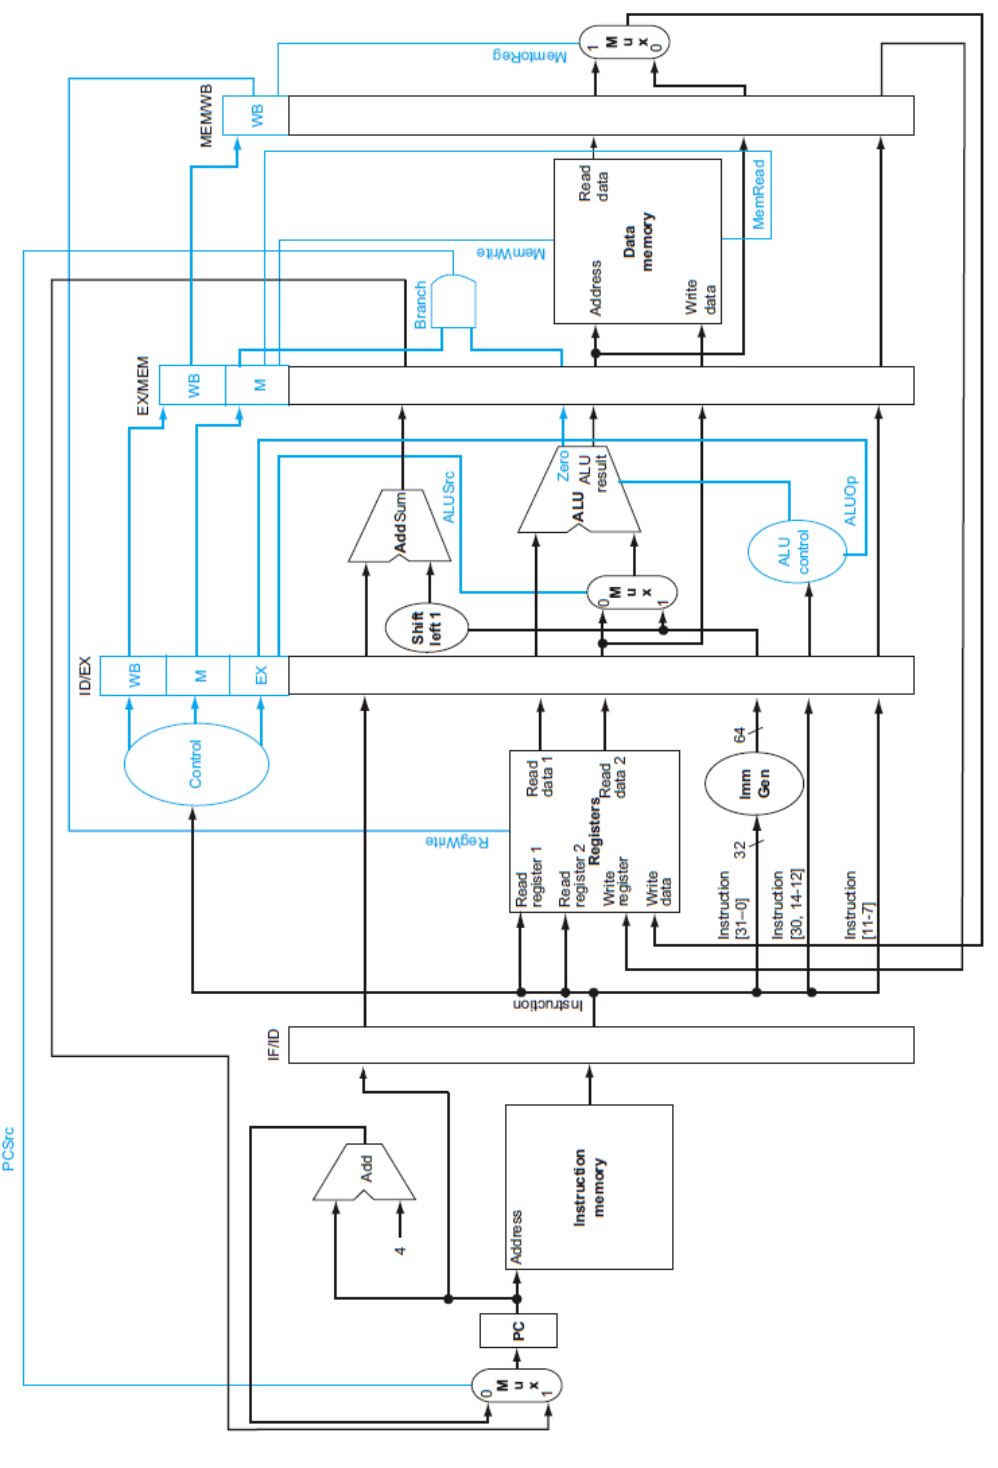
\includegraphics[scale=0.4,center]{./images/RISCV_arch.png}
			\caption{RISC-V architecture with four pipeline stage.}
			\label{fig:riscv_architecture1}
		\end{figure}  
		
	}% end RISC-V ISA
	
	\section{CV32E40P core}{
		CV32E40P is a 32-bit RISC-V core that implement RV32IM[F]C ISA using a custom extension called Xpulp, with this  extension the core is able to reach a high code density, performance and efficiency \bscite{NearThreshold1} \bscite{SlowSteadyWin}. The core architecture has been designed to work with a Near-Threshold voltage in order to increase the efficiency of the transistors.\\ 
		
		
		For this core are created some instruction extensions and architectural optimization that increase computational density and speed up processing reaching a 3.5x faster elaboration and 3.2x more energy efficiency. 
		This core has been designed also to be used in the Parellel Ultra Low Power (PULP) platform. PULP use a set of RISC-V core with shared memory to reach high efficiency, it contain a set of IP that enable this performances.\\
		
		
		The original name of the CV32E40P was OR10N based on the OpenRISC ISA, then in 2016 it change name in RI5CY and it became a RISC-V compatible core, it has been maintained by PULP Platform until 2020 when it begin to be contributed by OpenHW Group.\\
		
		In figure \ref{fig:cv32e40p_core_diagram} there is the main diagram of the CV32E40P core, it is a 4-stage in order RISC-V processor, the MULT block correspond to the M extension while compressed decoder is the C extension, in the figure there isn't the floating-point unit because it is optional in CV32E40P core.
		
	    \begin{figure}[H]
			\centering
			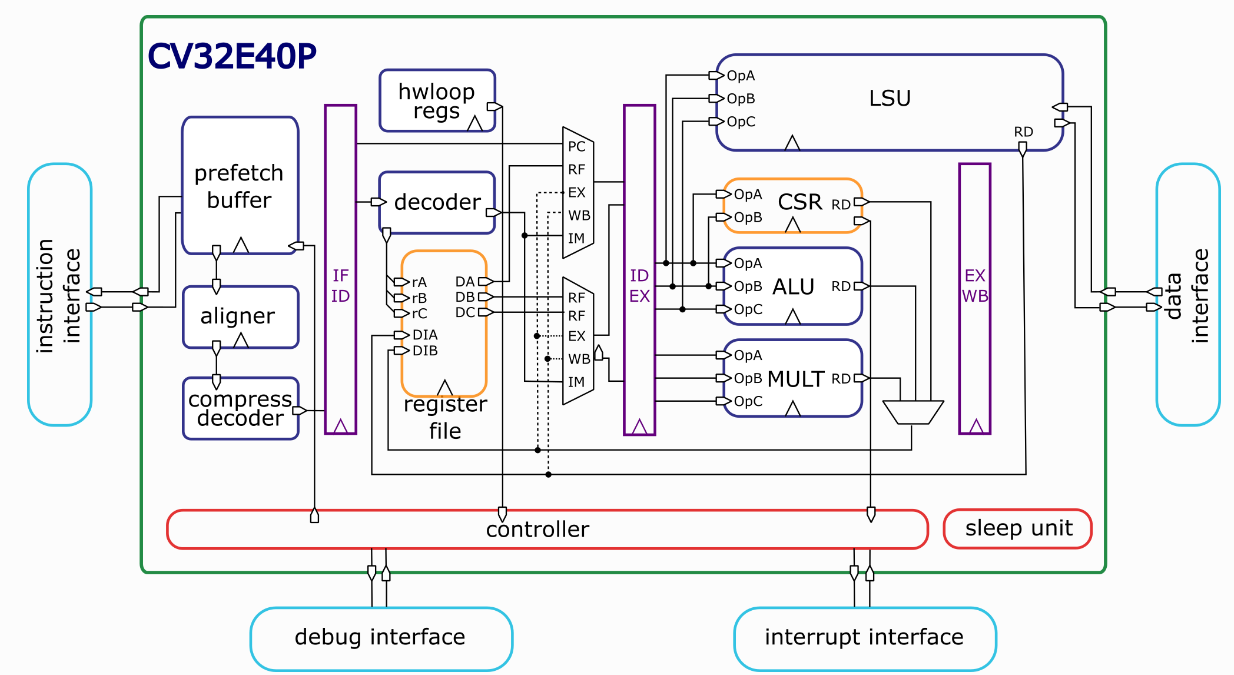
\includegraphics[scale=0.35,center]{./images/CV32E40P_core_diagram.png}
			\caption{CV32E40P core diagram.}
			\label{fig:cv32e40p_core_diagram}
		\end{figure}  
		
		In core repository \href{https://github.com/openhwgroup/cv32e40p}{cv32e40p} you can find all System Verilog code, documentation and verification procedures.
		This Master Thesis is focused on the transformation of the Instruction Fetch (IF) of the CV32E40P in a fault tolerant stage, for this reason we will focus on IF stage architecture of the core.
		
		\subsection{CV32e40P Instruction Fetch}{
		    The instruction fetch read the instruction from instruction memory and provide them to the Instruction Decode (ID).
		    As you can see in figure \ref{} the IF stage can be divided into six main block, anyway only  the Prefetch Buffer, the Compressed Decoder and the Aligner are designed as separate System Verilog file.
		    
		    \begin{figure}[H]
        		\centering
        		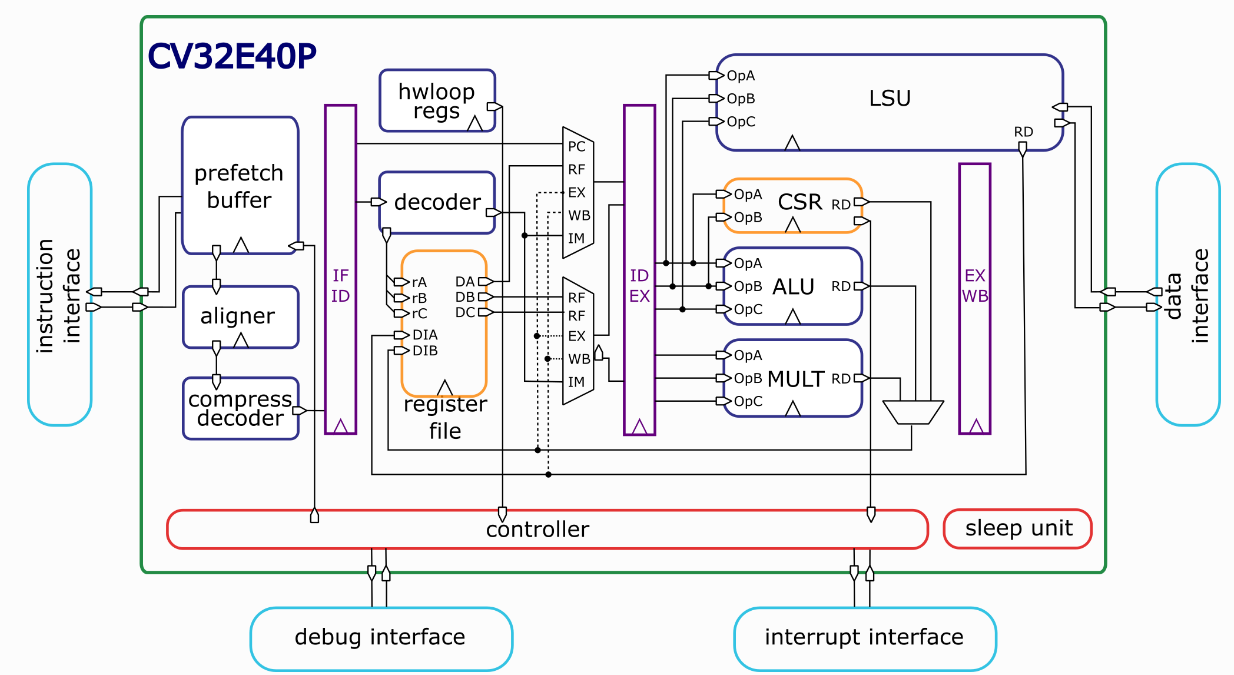
\includegraphics[scale=0.4,center]{./images/CV32E40P_core_diagram.png}
        		\caption{CV32E40P Instruction Fetch block diagram.}
        		\label{fig:cv32e40p_block_diagram}
        	\end{figure} 
        	
        	The six block of the IF stage cover these functions:
        	\begin{itemize}
        	    \item \textbf{Prefetch Buffer (PB):} PB is designed in order to fetch instruction from instruction memory/fetch via the OBI interface (cv32e40p\_obi\_interface.sv file), the instruction are then inserted to a four element FIFO (cv32e40p\_fifo.sv file) and then they are sent to the ID stage. OBI interface and the FIFO is controlled by the Prefetch Controller ( cv32e40p\_prefetch\_controller.sv file). 
        	    The advantage of the use of prefetch buffer is a higher instruction fetch speed that affects the core performances.
        	   
        	    \item \textbf{Compressed Decoder (CD):} CD check the instruction in order to verify if is compressed, this identification is done using the first two bit of the instruction, when they are both 1 means that the instruction isn't compressed and it is copied to the output, otherwise the instruction is decoded. 
        	    The stage is completely combinatory since it is described as a big case in System Verilog.
        	    
        	    \item \textbf{Aligner:} This block aligns instructions considering compressed instructions format. It contain an FSM and so FF components.
        	    
        	    \item \textbf{IF pipeline:} This block contain the pipeline of the if stage, it is a System Verilog (SV) block written inside the cv32e40p\_if\_stage.sv file.
        	    
        	    \item \textbf{IF FSM logic:} This block manage control signals of Prefetch Buffer and Aligner, it is a System Verilog (SV) block written inside the cv32e40p\_if\_stage.sv file.
        	    
        	    \item \textbf{Program Counter Definition (PCD):} PCD define the PC according to jump, branch, trap and exceptions. It is a System Verilog (SV) block written inside the cv32e40p\_if\_stage.sv file.
                
        	\end{itemize}
		}
		
	}% end cv32e40p Core

	%\section{FT RISC-V State Of Art}{
		
	%l}% end FT RISC-V State Of Art

}